\documentclass[letterpaper, onecolumn,10pt]{IEEEtran}

\usepackage{graphicx}
\usepackage{amssymb}
\usepackage{amsmath}
\usepackage{amsthm}

\usepackage{alltt}
\usepackage{float}
\usepackage{color}
\usepackage{url}
\usepackage{listings}
\usepackage{ifthen}


\usepackage[TABBOTCAP, tight]{}

\usepackage{geometry}
\geometry{textheight=8.5in, textwidth=6in}

%random comment

\newcommand{\cred}[1]{{\color{red}#1}}
\newcommand{\cblue}[1]{{\color{blue}#1}}

\usepackage{hyperref}
\usepackage{geometry}
\usepackage{caption}
\usepackage{url}
\usepackage{natbib}

\begin{document}
    \begin{titlepage}
    \newcommand{\HRule}{\rule{\linewidth}{0.5mm}}
    \center
    \textsc{\Large Oregon State University}\\[1.5cm]
    \textsc{\Large ST 314}\\[0.5cm]
    \textsc{\Large Summer 2019}\\[0.5cm]
    \HRule \\[0.4cm]
    { \huge \bfseries Data Analysis Three}\\[0.4cm] % Title of your document
    \HRule \\[1.5cm]
    \begin{minipage}{0.4\textwidth}
        \begin{flushleft} \large
        \emph{Author:}\\
        Thomas Noelcke
        \end{flushleft}
    \end{minipage}
    \begin{minipage}{0.4\textwidth}
        \begin{flushright} \large
        \emph{Instructor:} \\
        Katie Jager\\
        \end{flushright}
    \end{minipage}\\[2cm]
		\end{titlepage}
        
        \section{Part I}
            \subsection{Categorical Variable}
                The variable that I chose was the gaming device variable. I chose this variable because I'm interested in what proportion of people in this class are using which gaming devices. Below is a plot of the different gaming devices that people in this class are using.
                
                % Add Image of Gaming Devices Here
                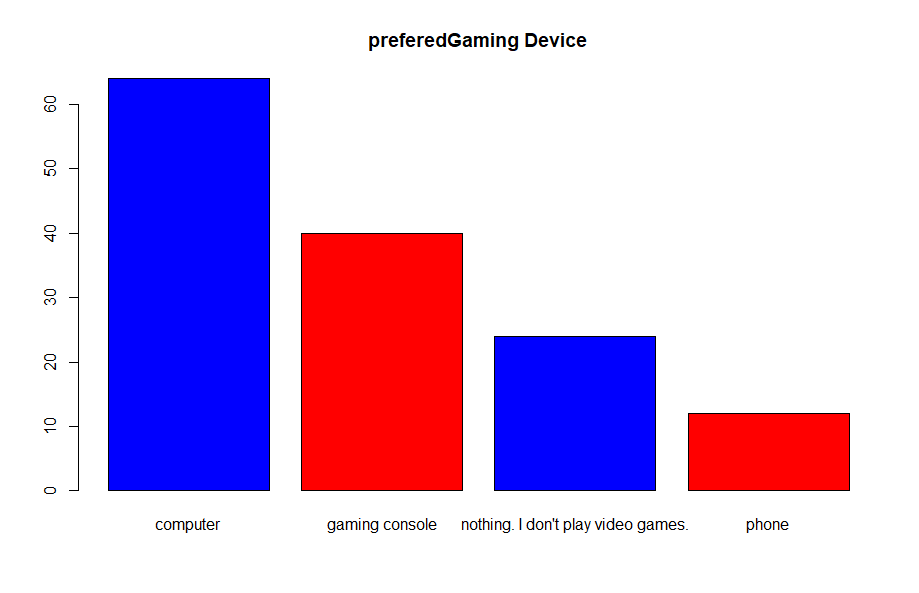
\includegraphics[width=\textwidth]{week3/Images/Histogram1.png}
                \begin{table}[H]
                    \begin{tabular}{|c|c|}
                        \textbf{Device} & \textbf{Count}\\
                        Computer & 64\\
                        Console & 40\\
                        I don't Game & 24\\
                        Phone & 12\\
                    \end{tabular}
                \end{table}
                The above plot once sorted from highest to lowest generally looks like it is linear in distribution. The gaming devices listed in order by popularity are, computer at 64 people , the console at 40, I don't game at 24, and lastly phone at 12. I was surprised by the number of people who don't game at all in comparison to the number of people that game on their phone. I thought that this would have been flip flopped.\\
                
            \subsection{Quantitative Variable}
                For my second variable I chose Gaming time in hours. I chose this variable because it complimented the categorical variable that I chose earlier. Below are images of the plots requested.\\
                
                %insert Histogram
                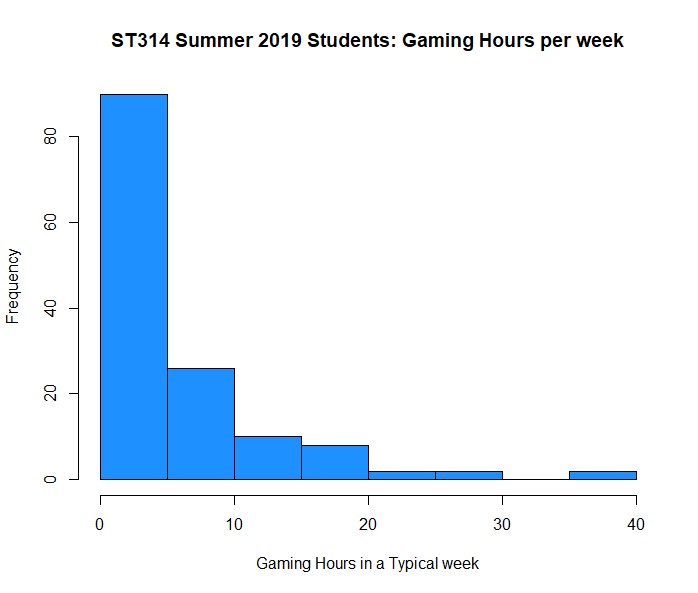
\includegraphics[width=\textwidth]{week3/Images/Histogram.png}
                
                %insert Box Plot
                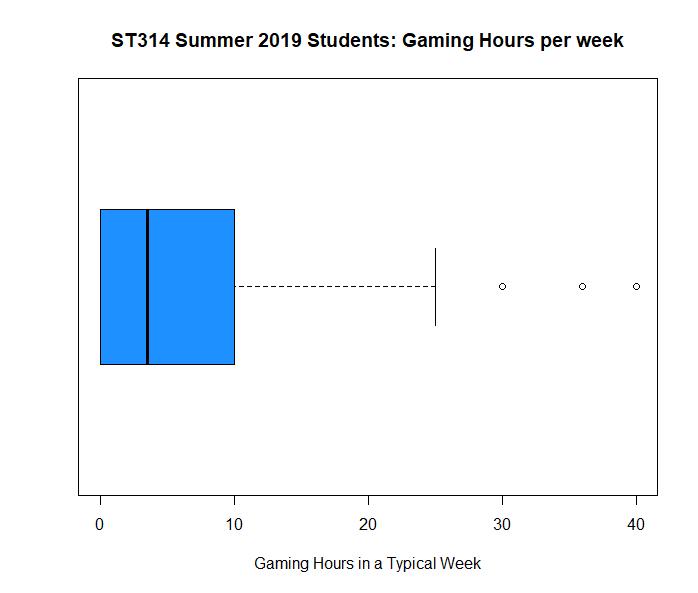
\includegraphics[width=\textwidth]{week3/Images/BoxPlot.png}
                
                I prefer the Histogram to visualize the data. I prefer this plot because it is more intuitive for me. It is also easier for me to tell which direction the plot is skewed if any. 
                
            
            \begin{table}[H]
                \begin{tabular}{|c|c|}
                    \textbf{Name} & \textbf{Value}\\
                    mean & 6.125\\
                    standard deviation & 7.768 \\
                    Minimum & 0.000\\
                    1st quartile & 0.000\\
                    median & 3.500\\
                    3rd quartile & 10.000\\
                    maximum & 40.000\\
                    IQR & 10.000\\
                \end{tabular}
            \end{table}
            
            With the given statistics and plots above we can say that the distribution of gaming hours is positively skewed. This is because the mean is much larger than the median but also because of the shape of the histogram. There were three outliers in this set of data that were between 25 and 40 hours. Given that we have skewed data with outliers that the median would be the preferred measurement for the center of the data. This is because the mean will be skewed higher due to the outliers in the data set.\\
            
            
        %How different are your sampled statistics in comparison to the overall class mean and standard deviation? How different is the distribution?   
        \section{Part 2}		
        %insert histogram and box plot belowwe
        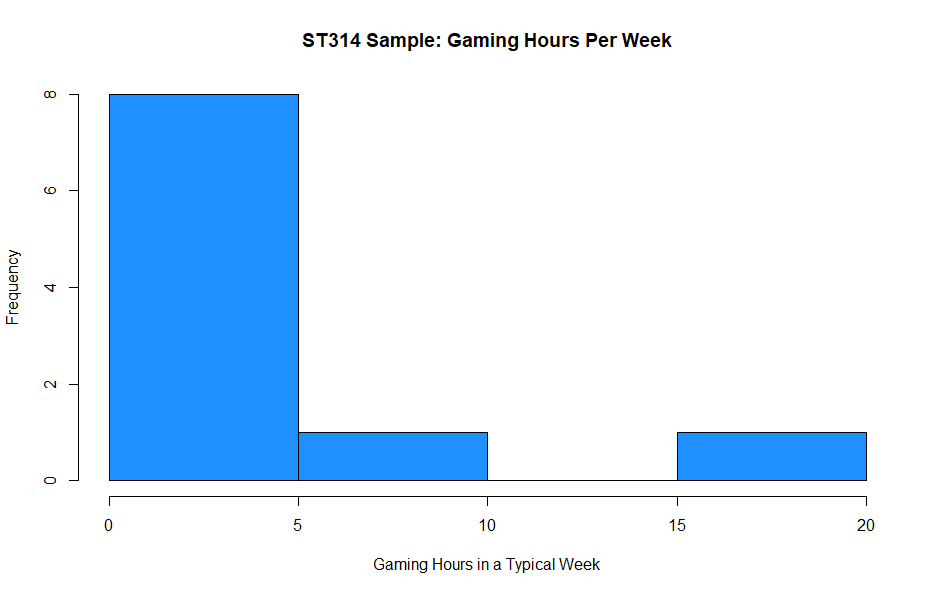
\includegraphics[width=\textwidth]{week3/Images/Histogram2.png}
        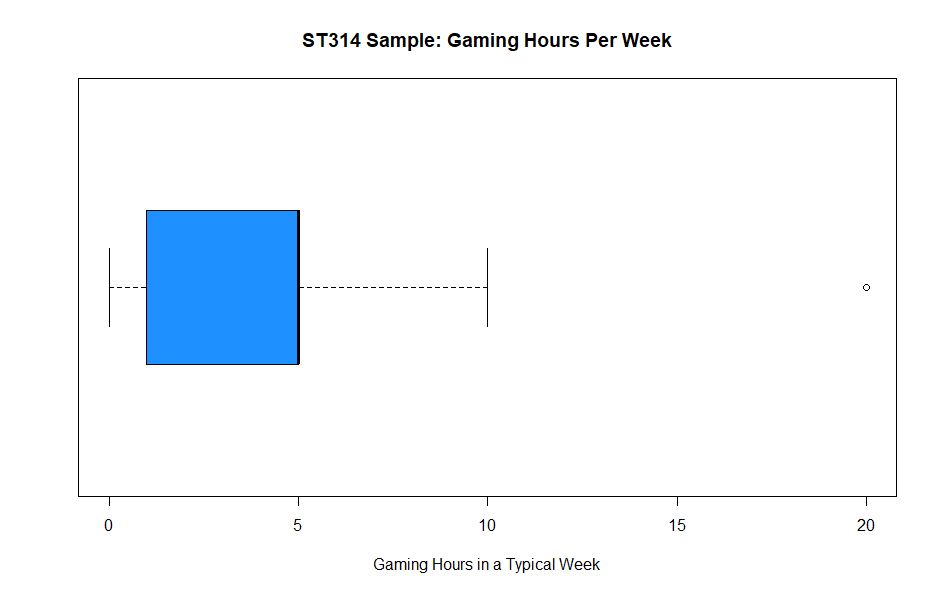
\includegraphics[width=\textwidth]{week3/Images/BoxPlot2.png}
        \begin{table}[H]
            \begin{tabular}{|c|c|}
                \textbf{Name} & \textbf{Value} \\
                 mean & 5.6\\
                 standard Deviation & 5.892\\
                 median & 5.0\\
            \end{tabular}
        \end{table}
        
        My sample values when compared to the population values were very different. The plot appeared to be positively skewed but looking closely and the mean and median they were fairly close for this sample. The box plot revealed that the mean was right at the top of the IQR indicating that the mean was skewed by an outlier. This is similar to the results for the population mean however the sample median and population median were very different. The standard deviation for the sample also differed from the population standard deviation.\\
        
        
		\end{document}